%! Author = thibaultchausson
%! Date = 23/07/2023

\subsection{Sujet}\label{subsec:sujet}

Le but de ce projet audiovisual est de réaliser de courtes vidéos appelé Reel sur Instagram, pour montrer la diversité de l'engagement associatif, mais plus particulièrement l'engagement des étudiant·e·s.

Le projet montrera divers moments de vie estudiantine, des interviews d'étudiant·e·s, pour promouvoir les activités dont il·elle·s sont responsable au sein de l'\gls{AE} \gls{UTBM}.

Ainsi, l'objectif principal de ce projet est de communiquer sur les différents événements de l'\gls{AE}, ainsi que ses temps fort, je peux citer de manière non exhaustive, le nouveau principe d'élection pour le Pôle Des Festivités (PDF), les soirées d'ampleurs co-réaliser avec les BDE de Belfort, mais encore promouvoir l'engagement dans l'association\ldots

Comme évoqué procurement, la motivation première de ce sujet est la promotion de la vie associative estudiantine.
Je suis motivé pour promouvoir l'\gls{AE} en lui donnant une autre image que celle actuelle, en montrant que derrière cette association tentaculaire, il y a des étudiant·e·s qui sont motivés pour améliorer le cadre de vie de leurs paires.
De plus, je trouve que donner la parole aux différents instigateur·trice·s de ces changements est d'autant plus gratifiant pour eux.

\subsection{Méthodes}\label{subsec:methodes}

\subsubsection{Le fond}

Comme évoqué précédement, je souhaite promouvoir l'engagement associatif, en particulier au sein de l'\gls{AE} de l'\gls{UTBM}.
Pour ce faire, je vais utiliser les personnes actives de cette association pour montrer leurs implications exemplaires dans divers domaines de cette grande association.

En d'autres mots, je veux donner envie aux autres étudiant·e·s que la vie associative de l'\gls{UTBM} est riche, et dynamique.

\subsubsection{La forme}

Pour mener à bien ce projet, j'ai décidé de réaliser de courtes capsules vidéos dynamiques de 1 à 1 minute 30, ce qui permet de garder mon auditoire attentif au message que je souhaite communiquer.
De ce fait, le format de Reels Instagram\footnote{Un Reel est une vidéo courte et divertisante de moins de 90 secondes (\href{https://about.instagram.com/fr-fr/features/reels}{Reels Instagram}).} correspond parfaitement à ces contraintes.

Les plates-formes numériques de communication en réseau ont révolutionné la façon dont nous communiquons, obtenons des informations et nous divertissons ; elles ont eu un impact majeur sur les nouvelles générations.
Nous pouvons remarquer que l'utilisation des réseaux sociaux a littéralement explosée avec la pandémie de COVID-19, ce qui peut s'expliquer par les divers confinements.
L'activité des nouvelles générations sur TikTok, Instagram a modifié les comportements sociaux de la génération actuelle.
Les likes, les commentaires et les abonnements stimulent le système de récompense dopaminergique, qui est la base des comportements addictifs\cite{pedrouzo2023hyperconnected}.
Ce qui implique une rétention plus importante des utilisateur·trice·s sur ces plateformes.
Ainsi, il parait pertinent de focaliser nos efforts sur ce mode de communication pour toucher et incité le plus d'étudiant·e·s de l'\gls{UTBM} à s'impliquer et à participer aux activités de l'Association des Étudiant·e·s de l'\gls{UTBM}.

Outre une rétention accrut des jeunes, Instagram donne les chiffres suivants : plus de 140 milliards de Reels visionnés sur Instagram et Facebook chaque jour\footnote{\href{https://business.instagram.com/instagram-reels?locale=fr_FR}{Faites-vous connaître avec Reels}}.

Comme j'utilise le format Reel d'Instagram, je dois me conformer à certaines règles, telles que\footnote{\href{https://about.instagram.com/fr-fr/features/reels}{Reels Instagram}} :
\begin{itemize}
    \item Le format de la vidéo est en 9/16
    \item La durée doit être comprise entre 15 à 90 secondes
    \item Utiliser des musiques libres de droit, ou intégrer directement les musiques proposées par Instagram
    \item Il faut prendre en compte les informations de l'interface Instagram qui peut cacher certains éléments du Reel (voir interface en Annexe la figure : \ref{fig:interfaceInsta})
\end{itemize}


Je peux lister différentes méthodes :
\begin{itemize}
    \item Vidéos d'illustration (avec ou sans bruit du fond)
    \item Vidéos présentées par l'instigateur du projet
    \item Animations
    \item Texte
    \item Icones
    \item Dessins
    \item Info-graphies
\end{itemize}

\subsection{Diagramme de Gantt}\label{subsec:diagramme-de-gantt}

Voici le diagramme de Gantt de début de projet :

\begin{figure}[!h]
    \begin{center}
        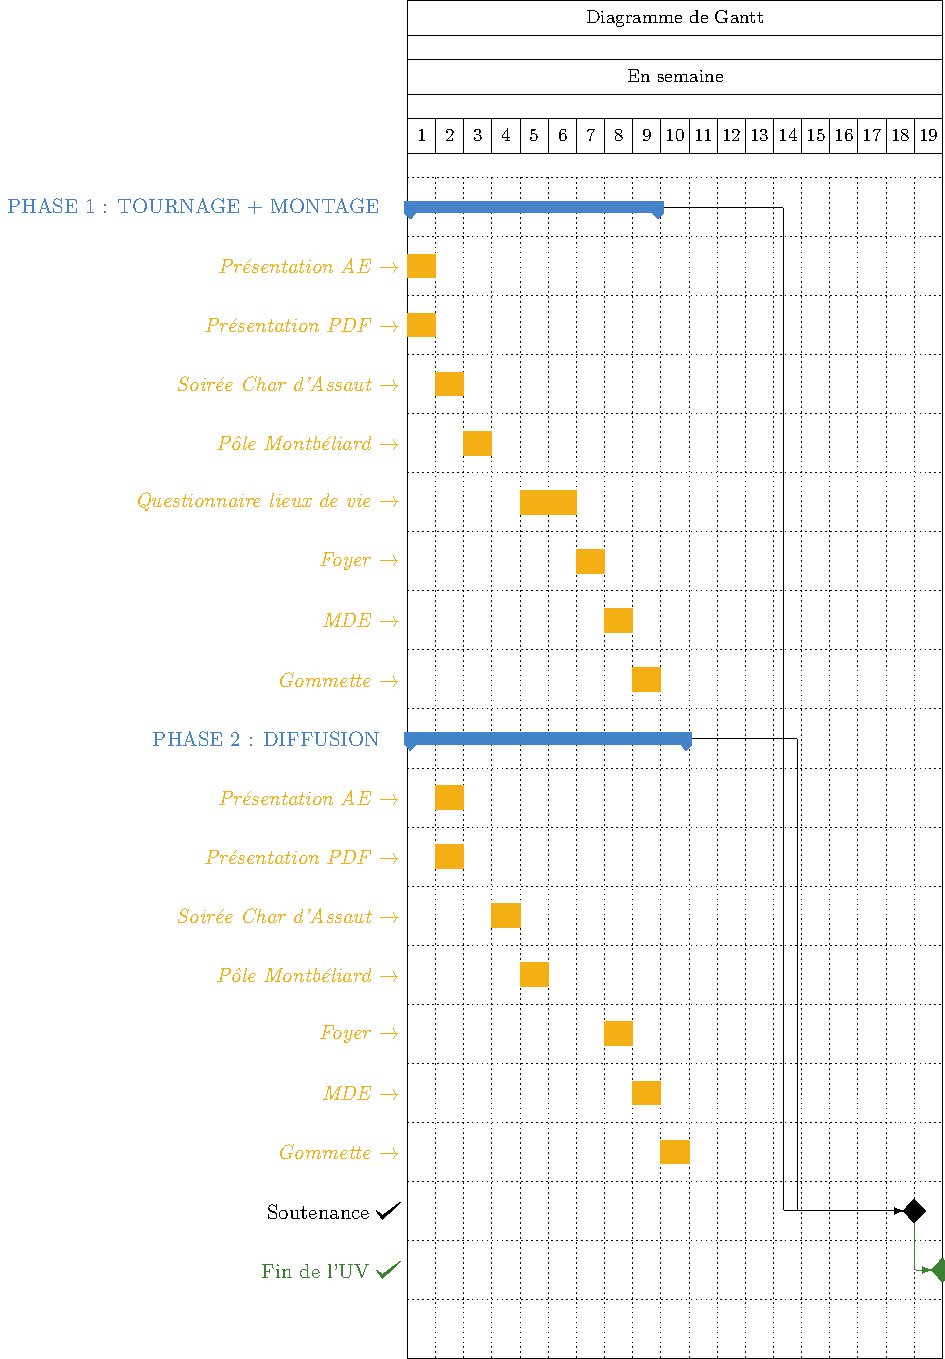
\includegraphics[scale=0.6]{ressources/gantt}
        \caption{Gantt initial \label{fig:ganttIni}}
    \end{center}
\end{figure}



L'objectif de ce projet est de réaliser rapidement des vidéos pour présenter l'association et les lieux de vie aux nouveaux·elles étudiant·e·s, ainsi je devais réaliser l'ensemble du tournage de ces vidéos en 9 semaines environs.

Comme dans tout projet, les délais sont très sensibles aux changements, j'ai eu quelques difficultés avec la prise de son, je devais emprunter les micros du Crunch Lab ce qui entrave la spontanéité des différents tournages.
En fin de projet l'\gls{AE} a décidé d'investir dans deux micros sans fil ce qui a permis de réaliser ma dernière vidéo plus facilement, ainsi que d'autre réalisation par le responsable communication de l'\gls{AE}.

De plus, la vidéo sur la présentation du Pôle Montbéliard n'a pas été réalisé, après discussion avec le président de l'\gls{AE} nous avons décidé de réaliser la présentation de la Gommette en même temps que le Pôle Montbéliard, sinon il y aurait eu des redites sur entre les deux vidéos.

Outre, ce choix de supprimer la vidéo de présentation de Montbéliard, des retards d'une ou deux semaines sur la fin du projet ont été constaté dû au fait des contraintes scolaires et personnelles des personnes devant présenter les différentes vidéos.

Dans une grande partie des objectifs des bases sont atteints.




